\chapter{Contribution}

This chapter is divided into multiple sections, which cover the architecture and the expandability of the implementation. The architecture is split into subsections covering the various components that were implemented throughout the thesis.

%Most important chapter of the thesis. Describes what the author contributes as research. Discusses intuition, motivation, describes and reasons about necessity of proposed elements. Defines theses based on reasonable assumptions. Discusses relevant aspects of contribution. Approximately 30 to 40 pages. Can be split into multiple chapters.

\section{Architecture}

The architecture is in the most classical way a microservice orientated architecture. Compared to a monolithic application there is a higher focus on single components and their implementation and therefore decouple the complexity in its entirety.

Services itself can be clustered into the "Distributed Crawler", "Distributed Analysis", "Database", and "Frontend" sections, whereas the database is a third party implementation that is built upon and integrated into the architecture. The visualization of the microservice architecture can be seen in \ref{fig:architecture}.

\todo{redo image with clustered sections}
\begin{figure}[H]
    \centering
    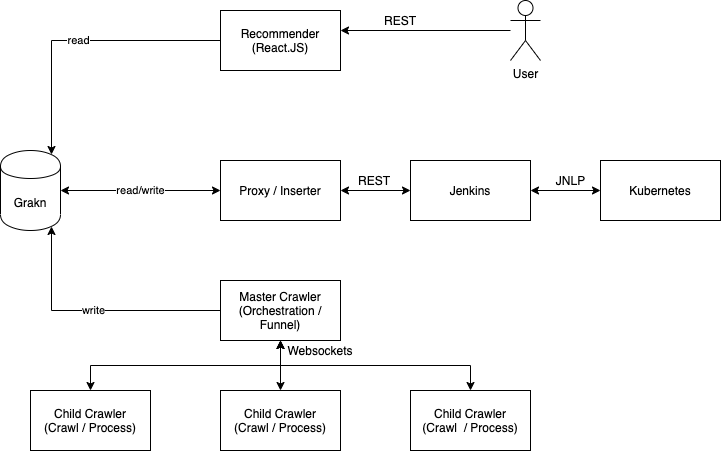
\includegraphics[scale=0.5]{graphics/architecture_v2.png}
    \caption{Architectural representation of the system as a whole}
    \label{fig:architecture}
\end{figure}

\subsection{Distributed Crawler}
First and foremost the main part of the implementation is the so-called "distributed crawler", which follows the master and node pattern, where one entity is the master that controls the spawned nodes. In this thesis, it can also be seen as orchestrator/information funnel and the crawling/processing unit. The reason for calling it a distributed crawler is that the overall function of this implementation can be seen as a crawler and distributed in the sense that the nodes can be distributed across multiple data centers or even be used on edge nodes with the appropriate implementation.

The implementation was done using Node.js, which is an asynchronous JavaScript runtime, which allows to run JavaScript outside of the browser and potentially build scalable applications. One of the big advantages of Node.js is that you can use the synergies of running JavaScript on the server-side and client-side. While this might not be the first thing that comes to mind when thinking about a distributed crawler, it does come in handy as a lot of services offer an API\footnote{Application Programming Interface} that returns JSON\footnote{JavaScript Object Notation} objects. Those JSON objects are easier to deal with in its native environment compared to other programming languages where one would rely on a third party implementation and a lot of serialization as the implementation was simply not meant for that environment.
As JavaScript runs in a JavaScript engine, the V8 engine developed by Google, it can be extended by creating C++ modules to make certain functions quicker as those would natively run on the system.

The master and crawler nodes are all based on one unified code base and the only difference between the two is the addition of the database connection and the orchestration routes, which are both parts of the master node. The default startup parameter for a node is to act as a crawler and connect to the master, which can be changed by setting one environment variable called "TYPE" to "master". The node would therefore load the database module, orchestration routes and use the master implementation of the communication channel instead of the crawler one.
The benefits of a unified code base are that the application could be extended in the future to support e.g. leader election or let the master act as a crawler as well. Meaning depending on the processing power provided the master could handle on top of its own capabilities the ones of a crawler as well and therefore provide more coverage of crawled sources.
Leader election quickly explained is that e.g. 4 spawned crawler would elect one of their own to be the master node, which often works based on either first come first serves basis or other defined constraints.

Master and node in itself are on a fundamental level just web servers providing a REST\footnote{Representational State Transfer} API, that allows one to trigger functions either from outside or from the application itself. REST comes along with well-defined methods using "GET", "POST", "DELETE", "PATCH", and some others. In the context of the distributed crawler, the most used methods are "GET" and "POST", as one either wants to receive information or in a sense add information, while often "POST" is used as well to incorporate functions that are not covered by the other methods.
While a REST API grants a good interface for a user or another application it is not very well suited for bidirectional real-time communication. As the crawlers are potentially distributed over various data-centers it can be tough to keep track of every single one of them, especially for the master as one would need e.g. a domain or another unique identifier to connect to all nodes prior to deploying the master. To counter this issue another communication channel was introduced the so-called WebSockets, which allows a real-time bidirectional communication where only the crawler would need to know the unique identifier of the master instead of the other way around. WebSockets initially coming from the web browser domain to allow client-server communication can also be used as a pure client-server communication without a web browser due to Node.js . WebSockets use a TCP socket to communicate through and are on the same OSI layer as HTTP and make use of channels that client and server have to subscribe to, to be able to send and receive messages about a specific topic. This bidirectional communication channel will be part of further subsections.

\subsubsection{Information funnel}
One of the functions of the master node is to act as an information funnel or proxy to the database. This makes the implementation of the crawler nodes easier as one does not have to worry about connecting to the database and can just use the bidirectional communication channel with the master. From a security point of view, it might also be easier to keep that one communication channel secure compared to multiple small ones to the database from depending on the setup of multiple locations.

Crawlers are essentially preparing and processing what they have crawled completely on their side and send the finished result to the master, which in return inserts the results into the database. The established bidirectional communication channel will be used keeping additional overhead small compared to other ways of implementing it.

\subsubsection{Orchestration}
As the master and node pattern already suggests controlling is one of the aspects of a master node. In this case, the job orchestration will be handled from the master node. Therefore the master provides a REST API that can be consumed by e.g. a user or some sort of automation like cron jobs that trigger crawling on a weekly basis. This could have been implemented using WebSockets as well, but a REST API is easier to consume compared to establishing a socket connection and then sending a message for a specific topic.

While orchestration is a REST API route it utilizes the WebSocket to send messages to its connected nodes and uses those as well for calculating windows that have to be crawled. A window in this sense is a range where the crawling should start and end, but more about the exact reasoning in the subsection about crawling. The orchestrator has a minimum and maximum value in between which should be crawled, which then in return is divided by the amount of crawler that are available at the point of receiving the request for orchestration. Each crawler therefore receives a window that should be covered.

\subsubsection{Crawling}
The implementation of the crawler makes use of the strategy pattern, which is a behavioral software pattern that allows selecting a strategy/implementation during runtime. This means in particular that there is a generic interface with the defined functions that have to be implemented by each strategy. In Node.js there is no classical object orientation that a lot of people might know from Java. Therefore the implementation makes use of a class that implements the generic interface that then each strategy can extend and implement. Further on there is one main class, which initializes the required strategy during runtime by making use of a simple switch case.

While this gives one a lot of flexibility and options to further extend this with other strategies it also brings along a couple of negative aspects like having to know which strategies are available and some extra effort into handling the implementation.

The first data source to be crawled and therefore the first strategy was for GitHub. GitHub is the biggest collection of public repositories and therefore offers a good starting point to cover roughly over a million deployment scripts in the case of docker-compose.
GitHub offers an API already in its third iteration with various REST endpoints that return JSON. One of those endpoints allows one to search through the code of all public repositories and therefore providing the starting point for the GitHub crawler strategy. As GitHub is quite popular and offers its API for free some of those API routes come with limitations, especially in something so resource-intensive as searching code through all public repositories.
Therefore the first limitation that GitHub introduced for the "search REST endpoint" is that only authorized users can use this function and with that, the second limitation comes along that requests will be limited to 30 per minute. To circumvent those two limitations each crawler gets assigned a designated GitHub Account with username and token to authenticate against the API and in case of running into the 30 requests per minute limit the crawler will sleep in intervals till the limit is lifted again.
The next limitation is that GitHub will only return a maximum of 1000 results per search query. While this seems difficult to bypass, GitHub brings along the proper tools to do so. One of the query parameters of the "GET" request is simply called "q" and allows one to build complex individual queries that are unique in itself and therefore offer up to 1000 results per query. The query parameter "q" can be extended to include the file name and file extension. Deployment scripts are often written in YAML\footnote{YAML Ain't Markup Language} and have come along with the extension ending "yaml" and "yml". Therefore doubles the number of search results in the case of YAML specific deployment scripts as one can vary between those two different spellings. The most important factor for circumventing the limit of 1000 results is to utilize the size of a file. GitHub allows one to define the size of a file, that you are searching for, in bytes or in a byte range, meaning one could search for all files in a range of 100-102 bytes or simple in the use case of the thesis to search per byte. This would allow one to create for the same file a unique query every single time.
Of course, GitHub has a limitation for this one as well and only allows to find files up to 384 Kilobyte, which in the context of this thesis is negligible as deployment scripts rarely touch the two-digit Kilobyte area.

Theoretically speaking 384 million files could be covered by just utilizing the size factor without even utilizing such things as extensions, order, or sorting. With those included depending on the type of deployment script, one could easily cover up to a billion search results.

To summarize the GitHub API, it comes along with a lot of limitations but at the same time with all tools needed to circumvent those limitations and therefore covering almost all public repositories.

This should give one a perspective as well on why one would utilize a distributed crawler as this allows to cover a much wider area much quicker by spawning more nodes. As previously mentioned in the part about orchestration a window area is defined for crawling, this is limited from 50 bytes to 384 Kilobytes as a 50 byte deployment script will most likely just include the very basics of its potential. One crawler does not cover the full range, except its the only crawler available, but rather the window that was set by the master node.

\subsubsection{Processing}


\subsubsection{Unified base}
\todo{meant as the same code base for client/server - interchangeable}
\subsection{Distributed Analysis}
\subsubsection{Choice of Tooling}
\todo{e.g. Jenkins + Kubernetes, conftest}
\subsubsection{Importance of Isolation}
\todo{e.g. CI and dind or kind}
\subsubsection{Vulnerability Scanning}
\subsubsection{Calculation of Score}
\subsubsection{Orchestrator / Funnel}
\todo{Normalization}
\todo{CVSS}
\subsection{Database - Grakn.ai}
\todo{Deduplication}
\subsubsection{Entity relationship model}
\subsubsection{Open Source Contributions}
\todo{e.g. own tooling for creating gexf compatible graphs - Limitations of provided tools (electron)}
\todo{e.g. own tooling for seeding the db model}
\subsection{Frontend}
\subsubsection{Content-based Recommendation}
\section{Expandability}
\todo{current focus on docker-compose, but can easily be extended to further sources, may it be crawling/processing/analysing/showing}
\section{IaC of implementation}

%\section{Open Source}
%\subsection{GitHub}

%\section{Architecture}
%\subsection{Microservices}
%\subsection{Software design pattern}
%\todo{Strategy pattern}
%\todo{Singleton}
%\subsection{Node.js}
%\subsection{React}

%\section{Protocols}
%\subsection{WebSocket}
%\subsection{REST}
%\subsection{gRPC}
%\subsection{JNLP}